\chapter{विद्युत और चुंबकीय क्षेत्रों में आवेशित कण}\label{ch:b1:charged-particles}

\cref{ch:b1:transient-regimes} के निशान खींचने वाले दोलनदर्शी के भीतर
इलेक्ट्रॉनों का कोई पुंज दो पट्टिकाओं के बीच के \omterm{def:b1:dc-circuits:voltage}{विभवांतर} से पर्दे पर इधर
से उधर हाँका जाता है; किसी \omterm{prop:b1:charged-particles:spectrometer}{द्रव्यमान वर्णक्रममापी} के चुंबक के भीतर दो समस्थानिकों
के आयन मिलीमीटरों भर अलग हो जाते हैं, क्योंकि एक दूसरे से आठ प्रतिशत भारी
है; और किसी अस्पताल के साइक्लोट्रॉन के भीतर प्रोटॉन दो सौ चक्करों तक बाहर
की ओर सर्पिल बनाते हैं और फिर प्रकाश की एक-तिहाई चाल से निकलकर किसी अर्बुद
को जला देते हैं। ये तीनों एक ही गतिकी हैं: किसी एकसमान क्षेत्र में --- चाहे
विद्युत हो या चुंबकीय --- कोई आवेश, और न्यूटन का नियम। यह अध्याय उसे हल
करता है --- \omterm{def:b1:charged-particles:lorentz}{विद्युत क्षेत्र} में परवलय, \omterm{def:b1:charged-particles:lorentz}{चुंबकीय क्षेत्र} में वृत्त और
कुंडलिनी --- और उसे उन यंत्रों में बदल देता है जो आवेशित कणों को छाँटते,
त्वरित करते और मापते हैं।

\begin{omfigure}
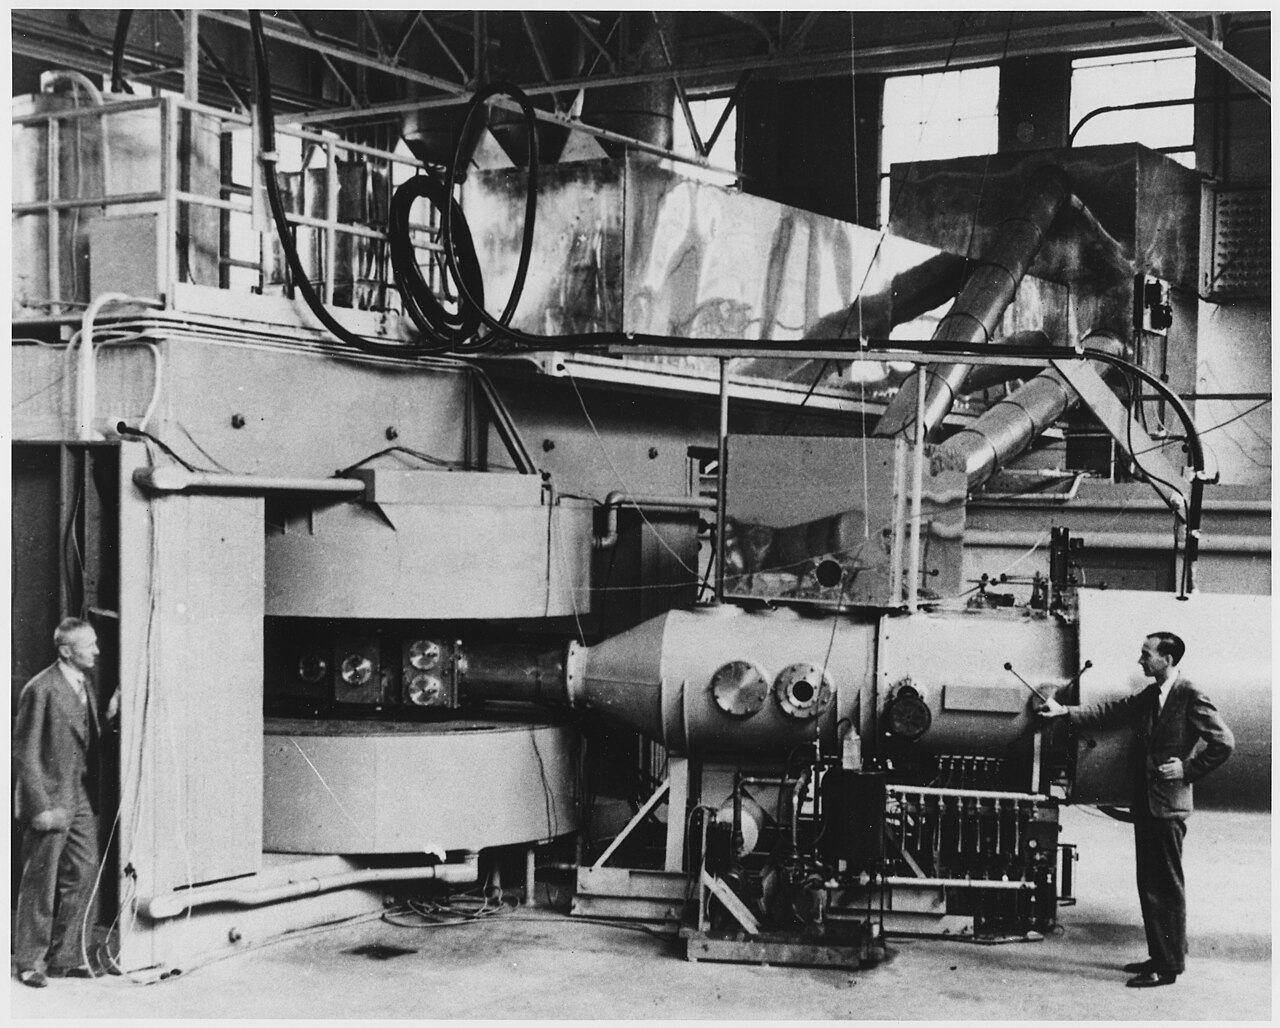
\includegraphics[width=0.60\linewidth]{images/book3/cyclotron-berkeley-60inch.jpg}

{\small बर्कली में लॉरेंस का 60-इंच साइक्लोट्रॉन, 1939 (अमेरिकी ऊर्जा विभाग): चुंबक के ध्रुवों के बीच प्रोटॉन बाहर की ओर सर्पिल बनाते हैं और हर चक्कर में दो बार धक्का पाते हैं, ठीक जैसा सप्ताहांत समस्या में है।}
\end{omfigure}

\section{लोरेंत्स बल}

\begin{definition}[लोरेंत्स बल]\label{def:b1:charged-particles:lorentz}
\index{लोरेंत्स बल}\index{विद्युत क्षेत्र}\index{चुंबकीय क्षेत्र}
आवेश $q$ का कोई कण, जो $\vect v$ वेग से किसी विद्युत क्षेत्र $\vect E$ और
किसी चुंबकीय क्षेत्र $\vect B$ में चल रहा हो, यह बल पाता है
\[
\vect F = q\big(\vect E + \vect v\wedge\vect B\big) .
\]
विद्युत भाग $\vect E$ के अनुदिश होता है ($q < 0$ के लिए उसके विपरीत) और गति
से स्वतंत्र रहता है; चुंबकीय भाग $\vect v$ और $\vect B$ दोनों पर लंब होता
है, चाल के समानुपाती होता है, और विराम में पड़े किसी कण के लिए लुप्त हो
जाता है। मात्रक: $\vect E$ \unit{V/m} में (या \unit{N/C} में), और $\vect B$
टेस्ला में (\unit{T}): $\qty{1}{T} = \qty{1}{N/(A.m)}$।
\end{definition}

\begin{proposition}[लोरेंत्स बल का कार्य]\label{prop:b1:charged-particles:work}
चुंबकीय बल कोई कार्य नहीं करता: उसकी शक्ति $q(\vect v\wedge\vect B)\cdot\vect v$
शून्य है, अतः अकेला \omterm{def:b1:charged-particles:lorentz}{चुंबकीय क्षेत्र} वेग की दिशा तो बदल देता है, पर चाल या
\omterm{thm:b1:work-and-energy:ke}{गतिज ऊर्जा} कभी नहीं। विद्युत बल की शक्ति
$q\vect E\cdot\vect v$ है, और दो बिंदुओं के बीच उसका कार्य $q(V_A - V_B) =
qU_{AB}$ है (\cref{ch:b1:potential-capacitors}): यानी आवेश $q$ का कोई कण
\omterm{def:b1:dc-circuits:voltage}{विभवांतर} $U$ पार करके \omterm{thm:b1:work-and-energy:ke}{गतिज ऊर्जा} $\abs{qU}$ पा लेता है।
\end{proposition}

\begin{proof}
$\vect v\wedge\vect B \perp \vect v$। स्थिरवैद्युत क्षेत्र विभव से व्युत्पन्न
होता है, $\vect E = -\overrightarrow{\operatorname{grad}}V$, अतः $q\vect E$
संरक्षी है और उसकी $E_p = qV$ है।
\end{proof}

\begin{definition}[इलेक्ट्रॉन-वोल्ट]\label{def:b1:charged-particles:eV}
\index{इलेक्ट्रॉन-वोल्ट}
\emph{इलेक्ट्रॉन-वोल्ट} वह \omterm{thm:b1:work-and-energy:ke}{गतिज ऊर्जा} है जो कोई मूल आवेश एक वोल्ट पार करके
पाता है: $\qty{1}{eV} = \qty{1.60e-19}{J}$। रसायन कुछ \unit{eV} पर रहता
है, X-किरण नलिकाएँ दसियों \unit{keV} पर, नाभिकीय भौतिकी \unit{MeV} पर, और
कण-भौतिकी \unit{GeV} तथा \unit{TeV} पर।
\end{definition}

\begin{remark}[गुरुत्व की उपेक्षा क्यों]\label{rem:b1:charged-particles:gravity}
\qty{1}{kV/m} के क्षेत्र में किसी इलेक्ट्रॉन के लिए --- जो प्रयोगशाला का
एक साधारण मान है --- विद्युत बल $eE = \qty{1.6e-16}{N}$ है, जबकि भार
$mg = \qty{9e-30}{N}$: यानी $10^{13}$ गुना छोटा। इस अध्याय की हर गणना से
भार बिना दुबारा सोचे हटा दिया जाता है। (आपेक्षिक सीमा दूसरी बात है: नीचे
के सूत्र $\tfrac12 mv^2 \ll mc^2$ के लिए ही सही हैं, अर्थात् इलेक्ट्रॉनों
के लिए लगभग \qty{50}{keV} से नीचे और प्रोटॉनों के लिए \qty{100}{MeV} से
नीचे; देखिए वर्ष 3 का खंड।)
\end{remark}

\section{एकसमान विद्युत क्षेत्र}

\begin{proposition}[त्वरण और विक्षेपण]\label{prop:b1:charged-particles:efield}
\index{त्वरक विभवांतर}
किसी एकसमान क्षेत्र $\vect E$ में त्वरण $\vect a = q\vect E/m$ अचर रहता है:
अतः गति ठीक किसी प्रक्षेप्य जैसी होती है, जिसमें $q\vect E/m$ $\vect g$
की जगह ले लेता है।
\begin{itemize}
  \item विराम से छोड़कर किसी \omterm{def:b1:dc-circuits:voltage}{विभवांतर} $U$ से त्वरित किया गया कण
        $v = \sqrt{2\abs{qU}/m}$ तक पहुँचता है।
  \item $v_0$ चाल से $x$ के अनुदिश ऐसे किसी $L$ लंबाई के क्षेत्र में
        घुसने पर जहाँ $\vect E = E\vect e_y$ है, वह परवलय
        $y = (qE/2mv_0^2)x^2$ पर चलता है और $\alpha$ कोण से विक्षेपित होकर
        निकलता है, जहाँ $\tan\alpha =
        qEL/mv_0^2$, मानो वह पट्टिकाओं के बीचोंबीच से सीधी रेखा में आया
        हो।
\end{itemize}
\end{proposition}

\begin{proof}
ऊर्जा: $\tfrac12 mv^2 = \abs{qU}$। विक्षेपण: $x = v_0t$, $y =
\tfrac12(qE/m)t^2$; निर्गम पर $\dd y/\dd x = (qE/m)(x/v_0^2)$ को
$L$ पर लीजिए; और निर्गम पर स्पर्शरेखा $y = (qEL/mv_0^2)(x - L/2)$ अक्ष को
$x = L/2$ पर काटती है।
\end{proof}

\begin{omfigure}
\begin{tikzpicture}[font=\small, x=1cm, y=1cm]
  \draw[thick] (0,1.1) -- (3.6,1.1); \draw[thick] (0,-1.1) -- (3.6,-1.1);
  \node[above] at (1.8,1.1) {$-$}; \node[below] at (1.8,-1.1) {$+$};
  \draw[-Stealth, omDef] (1.2,-0.85) -- (1.2,0.85) node[midway, left] {$\vect E$};
  \draw[-Stealth, omThm, thick] (-1.6,0) -- (0,0) node[pos=0.3, above] {$v_0$};
  \draw[omThm, thick, domain=0:3.6, samples=50] plot (\x, {-0.06*\x*\x});
  % exit at x=3.6: y=-0.778, slope=-0.432
  \draw[-Stealth, omThm, thick] (3.6,-0.778) -- (6.4,{-0.778-0.432*2.8});
  \draw[dashed, omExo] (1.8,0) -- (6.4,{-0.432*4.6});
  \draw[dashed] (-0.2,0) -- (6.6,0);
  \draw (5.0,0) arc (0:-23.4:1.4); \node at (5.4,-0.35) {$\alpha$};
  \draw[thick] (7.0,-2.4) -- (7.0,1.2); \node[above] at (7.0,1.2) {पर्दा};
  \fill[omThm] (7.0,{-0.778-0.432*3.4}) circle (1.8pt);
  \draw[Stealth-Stealth] (0,1.5) -- (3.6,1.5) node[midway, above] {$L$};
  \node[omExo, font=\footnotesize, below] at (1.8,-0.05) {$L/2$};
  \fill (1.8,0) circle (1.2pt);
\end{tikzpicture}

{\small स्थिरवैद्युत विक्षेपण: पट्टिकाओं के बीच इलेक्ट्रॉन (यहाँ
$q < 0$, इसलिए धनात्मक पट्टिका की ओर विक्षेपित) किसी परवलय पर चलता है; और
उनके आगे वह सीधा उड़ता है, मानो पट्टिकाओं के मध्यबिंदु से आ रहा हो
--- यही कैथोड-किरण दोलनदर्शी की ज्यामिति है।}
\end{omfigure}

\begin{example}[दोलनदर्शी की नलिका]\label{ex:b1:charged-particles:crt}
$U_0 = \qty{2.0}{kV}$ से त्वरित इलेक्ट्रॉन ($v_0 = \qty{2.65e7}{m/s}$, यानी
$c$ का दसवाँ भाग --- बस आपेक्षिक होने से पहले) \qty{4.0}{cm} लंबी और
\qty{1.0}{cm} की दूरी पर रखी उन पट्टिकाओं को पार करते हैं जिन पर
\qty{100}{V} है: $E = \qty{1.0e4}{V/m}$,
$\tan\alpha = eEL/mv_0^2 = EL/2U_0 = 0.10$, और पट्टिकाओं के केंद्र से
\qty{30}{cm} आगे रखे पर्दे पर बिंदु \qty{3.0}{cm} खिसक जाता है --- यानी
\qty{0.3}{mm} प्रति वोल्ट, जो नलिका की सुग्राहिता है, और जो पूरी तरह
ज्यामिति तथा \omterm{prop:b1:charged-particles:efield}{त्वरक विभवांतर} से तय होती है।
\end{example}

\section{एकसमान चुंबकीय क्षेत्र}

\begin{theorem}[एकसमान चुंबकीय क्षेत्र में गति]\label{thm:b1:charged-particles:bfield}
\index{साइक्लोट्रॉन गति}\index{लार्मर त्रिज्या}\index{साइक्लोट्रॉन आवृत्ति}\index{कुंडलिनी गति}
आवेश $q$, द्रव्यमान $m$ और वेग $\vect v_0$ वाला कोई कण, जिसका वेग किसी
एकसमान $\vect B$ पर लंब हो, अचर चाल $v_0$ से ऐसा वृत्त खींचता है जिसकी
त्रिज्या और \omterm{def:b1:wave-propagation:signal}{कोणीय आवृत्ति} हैं
\[
R = \frac{mv_0}{\abs q B}, \qquad \omega_c = \frac{\abs q B}{m},
\]
जहाँ \emph{\omterm{thm:b1:charged-particles:bfield}{साइक्लोट्रॉन आवृत्ति}} $\omega_c$ चाल से स्वतंत्र है; और घूर्णन
की दिशा $q$ के चिह्न पर निर्भर करती है। यदि $\vect v_0$ में कोई घटक
$v_\parallel$ भी हो, जो $\vect B$ के अनुदिश हो, तो वह घटक अपरिवर्तित रहता है और \omterm{def:b1:point-kinematics:frame}{गतिपथ}
$mv_\perp/\abs qB$ त्रिज्या तथा $2\pi mv_\parallel/\abs qB$ पिच वाली एक
\emph{कुंडलिनी} होती है, जो क्षेत्र-रेखाओं के चारों ओर लिपटी रहती है।
\end{theorem}

\begin{proof}
बल $q\vect v\wedge\vect B$ $\vect v$ पर और $\vect B$ पर लंब है; चाल अचर है
(कोई कार्य नहीं) और $\vect B$ के अनुदिश घटक पर कोई बल नहीं लगता।
$\vect B$ पर लंब तल में बल का परिमाण अचर $\abs qv_\perp B$ है, और वह सदा
वेग पर लंब रहता है: यानी एकसमान \omterm{cor:b1:point-kinematics:circular}{वृत्तीय गति}
(\cref{thm:b1:point-kinematics:frenet}), जिसमें $mv_\perp^2/R =
\abs qv_\perp B$। तब $\omega_c = v_\perp/R$; और आवर्तकाल $2\pi m/\abs qB$ को
$v_\parallel$ से गुणा करने पर पिच मिलती है।
\end{proof}

\begin{omfigure}
\begin{tikzpicture}[font=\small, x=1cm, y=1cm]
  % circle in a plane, B out of page
  \foreach \x in {-1.8,-0.6,0.6,1.8} \foreach \y in {-1.8,-0.6,0.6,1.8} {\draw (\x,\y) circle (0.07); \fill (\x,\y) circle (0.8pt);}
  \node[omDef, right] at (2.1,2.25) {$\vect B$ (पन्ने से बाहर)};
  \draw[omThm, thick] (0,0) circle (1.3);
  \fill[omThm] (1.3,0) circle (1.6pt);
  \draw[-Stealth, omThm, thick] (1.3,0) -- (1.3,1.1) node[right] {$\vect v$};
  \draw[-Stealth, omDef, thick] (1.3,0) -- (0.3,0) node[below, pos=0.6] {$q\vect v\wedge\vect B$};
  \node[omThm, font=\footnotesize] at (0,-2.3) {$R = \dfrac{mv}{\abs qB}$};
  % helix on the right
  \begin{scope}[xshift=6.5cm]
  \draw[-Stealth, omDef, thick] (-0.4,-2.2) -- (-0.4,2.4) node[above] {$\vect B$};
  \draw[omThm, thick, domain=0:12.57, samples=200, variable=\t] plot ({0.9*cos(deg(\t))+1.0},{0.16*\t-2.0+0.3*sin(deg(\t))});
  \node[omThm, font=\footnotesize, right] at (2.0,-0.2) {पिच $2\pi mv_\parallel/\abs qB$};
  \end{scope}
\end{tikzpicture}

{\small बाएँ: जिस आवेश का वेग $\vect B$ पर लंब है वह \omterm{thm:b1:charged-particles:bfield}{साइक्लोट्रॉन आवृत्ति}
$\abs qB/m$ से चक्कर लगाता है, और चुंबकीय बल \omterm{cor:b1:point-kinematics:circular}{अभिकेंद्र त्वरण} देता है।
दाएँ: $\vect B$ के अनुदिश वेग-घटक होने पर कोई कुंडलिनी क्षेत्र-रेखा के
चारों ओर लिपट जाती है --- यही पृथ्वी के क्षेत्र में फँसे इलेक्ट्रॉनों की
गति है।}
\end{omfigure}

\begin{example}[परिमाण की कोटियाँ]\label{ex:b1:charged-particles:orders}
\qty{1}{mT} में \qty{1}{keV} का कोई इलेक्ट्रॉन ($v = \qty{1.9e7}{m/s}$):
$R = \qty{11}{cm}$, $\omega_c = \qty{1.8e8}{rad/s}$, और एक चक्कर
\qty{36}{ns} में --- हर ऊर्जा पर वही आवर्तकाल, और यही साइक्लोट्रॉन को
संभव बनाता है। पृथ्वी के \qty{50}{\micro T} में सौर पवन का कोई प्रोटॉन
(\qty{1}{keV}, \qty{4.4e5}{m/s}): $R = \qty{92}{m}$; वह क्षेत्र-रेखाओं को
पार नहीं कर सकता, केवल उनके अनुदिश ध्रुवों की ओर सर्पिल बना सकता है ---
यही ध्रुवीय ज्योति है।
\end{example}

\section{यंत्र}

\begin{proposition}[वेग चयनक और द्रव्यमान वर्णक्रममापी]\label{prop:b1:charged-particles:spectrometer}
\index{वेग चयनक}\index{द्रव्यमान वर्णक्रममापी}
एक-दूसरे को काटते एकसमान क्षेत्रों $\vect E \perp \vect B$ में, दोनों पर लंब
चलता कोई कण बिना विक्षेपित हुए तभी निकलता है जब $v = E/B$ हो, उसका आवेश और
द्रव्यमान चाहे जो हो (\emph{\omterm{prop:b1:charged-particles:spectrometer}{वेग चयनक}})। अकेले \omterm{def:b1:charged-particles:lorentz}{चुंबकीय क्षेत्र} में ज्ञात
चाल का कोई कण $2mv/\abs qB$ व्यास का अर्धवृत्त खींचता है: उसे नापने पर
$m/q$ मिल जाता है (\emph{\omterm{prop:b1:charged-particles:spectrometer}{द्रव्यमान वर्णक्रममापी}})। किसी \omterm{def:b1:dc-circuits:voltage}{विभवांतर} $U$ से
त्वरित आयन, जब $B$ में मोड़े जाएँ, यहाँ गिरते हैं
\[
R = \frac{1}{B}\sqrt{\frac{2mU}{\abs q}} :
\]
जहाँ $m$ और $m + \Delta m$ द्रव्यमान वाले दो समस्थानिक $\Delta R \approx
R\,\Delta m/2m$ भर अलग हो जाते हैं।
\end{proposition}

\begin{proof}
$q\vect E + q\vect v\wedge\vect B = \vect 0$ के लिए ठीक दिशा के साथ $vB = E$
चाहिए। $R = mv/qB$, जहाँ $v = \sqrt{2qU/m}$; अब
$\ln R = \tfrac12\ln m + \text{नियतांक}$ का अवकलन कीजिए।
\end{proof}

\begin{example}[कार्बन के समस्थानिक]\label{ex:b1:charged-particles:isotopes}
\qty{20}{kV} से त्वरित एकल आवेशित $^{12}$C और $^{13}$C आयन \qty{0.50}{T}
में: $R = \qty{14.1}{cm}$ और \qty{14.7}{cm}, यानी \qty{5.8}{mm} की दूरी पर
--- संसूचक पर दो अलग बिंदु, और उनकी तीव्रताओं का अनुपात ही समस्थानिक
बहुलता है, जो रेडियोकार्बन तिथि-निर्धारण और हर समस्थानिक विश्लेषण का कच्चा
माल है।
\end{example}

\begin{proposition}[साइक्लोट्रॉन]\label{prop:b1:charged-particles:cyclotron}
\index{साइक्लोट्रॉन}
किसी एकसमान $\vect B$ में दो खोखले अर्ध-बेलन (``डी''), और उनके बीच
\omterm{thm:b1:charged-particles:bfield}{साइक्लोट्रॉन आवृत्ति} पर कोई प्रत्यावर्ती \omterm{def:b1:dc-circuits:voltage}{विभवांतर} $U$: कण हर डी के भीतर
चक्कर लगाता है (वहाँ कोई क्षेत्र नहीं), प्रति चक्कर दोनों अंतराल-पारों में
से हर एक पर $\abs qU$ से त्वरित होता है, और $R \propto v$ के साथ बाहर की ओर
सर्पिल बनाता है; निष्कर्षण त्रिज्या $R_{\max}$ पर उसकी \omterm{thm:b1:work-and-energy:ke}{गतिज ऊर्जा} है
\[
E_k = \frac{q^2B^2R_{\max}^2}{2m},
\]
जो \omterm{def:b1:dc-circuits:voltage}{विभवांतर} से स्वतंत्र है, और \omterm{def:b1:dc-circuits:voltage}{विभवांतर} केवल चक्करों की संख्या तय करता है।
\end{proposition}

\begin{proof}
चूँकि $\omega_c$ चाल पर निर्भर नहीं करता, इसलिए नियत आवृत्ति का \omterm{def:b1:dc-circuits:voltage}{विभवांतर}
चक्कर दर चक्कर कण के साथ ताल में बना रहता है; और $v = \abs qBR/m$, जहाँ
त्रिज्या $R$ है।
\end{proof}

\begin{omfigure}
\begin{tikzpicture}[font=\small, x=1cm, y=1cm]
  \draw[thick, omDef] (0,0) ++(95:2.4) arc (95:265:2.4);
  \draw[thick, omDef] (0,0) ++(-85:2.4) arc (-85:85:2.4);
  \draw[thick, omDef] (-0.2,2.4) -- (-0.2,-2.4); \draw[thick, omDef] (0.2,2.4) -- (0.2,-2.4);
  \node[omDef] at (-1.6,1.9) {डी}; \node[omDef] at (1.6,1.9) {डी};
  \node[above] at (0,2.5) {$U\cos\omega_ct$};
  \draw[omThm, thick, domain=0:1440, samples=300, variable=\t] plot ({(0.15+0.0011*\t)*cos(\t)},{(0.15+0.0011*\t)*sin(\t)});
  \draw[-Stealth, omThm, thick] ({(0.15+0.0011*1440)*cos(1440)},{(0.15+0.0011*1440)*sin(1440)}) -- ++(0.9,0.0);
  \foreach \x in {-1.7,-0.9,0.9,1.7} \foreach \y in {-1.7,-0.9,0.9,1.7} {\draw (\x,\y) circle (0.06); \fill (\x,\y) circle (0.7pt);}
  \node[right] at (2.5,-1.0) {$\vect B$ पन्ने से बाहर};
  \node[omThm, font=\footnotesize] at (3.3,0.3) {निष्कर्षण};
\end{tikzpicture}

{\small साइक्लोट्रॉन: किसी एकसमान \omterm{def:b1:charged-particles:lorentz}{चुंबकीय क्षेत्र} में दो डी; कण डियों के
भीतर चक्कर लगाता है और अंतराल के \omterm{def:b1:dc-circuits:voltage}{विभवांतर} से प्रति चक्कर दो बार धक्का पाता
है, वह भी सदा समकला में, क्योंकि उसका आवर्तकाल उसकी चाल पर निर्भर नहीं
करता। कोर पर ऊर्जा केवल $B$ और त्रिज्या पर निर्भर है।}
\end{omfigure}

\begin{example}[अस्पताल का साइक्लोट्रॉन]\label{ex:b1:charged-particles:medical}
प्रोटॉन, $B = \qty{1.5}{T}$, $R_{\max} = \qty{0.50}{m}$: $E_k =
(1.6\times10^{-19} \times 1.5 \times 0.5)^2/(2 \times 1.67\times10^{-27}) =
\qty{4.3e-12}{J} = \qty{27}{MeV}$, और $f_c = \omega_c/2\pi = \qty{23}{MHz}$
पर। डियों पर \qty{50}{kV} के साथ प्रति चक्कर \qty{100}{keV}: यानी
\qty{12}{\micro s} में $270$ चक्कर। कुछ दसियों \unit{MeV} से ऊपर द्रव्यमान की
आपेक्षिक वृद्धि (वर्ष 3 का खंड) प्रोटॉनों की ताल बिगाड़ देती है; इसलिए
\qty{230}{MeV} की चिकित्सा-मशीनें आवृत्ति या क्षेत्र को घटा-बढ़ाकर भरपाई
करती हैं --- यही सप्ताहांत समस्या का विषय है।
\end{example}

\begin{proposition}[हॉल प्रभाव]\label{prop:b1:charged-particles:hall}
\index{हॉल प्रभाव}
$d$ मोटाई की कोई पट्टी, जिसमें धारा $I$ बह रही हो और जिसके वाहकों का आवेश
$q$ तथा घनत्व $n$ हो, और जो पट्टी पर लंब किसी क्षेत्र $B$ में रखी हो, अपनी
चौड़ाई के दोनों किनारों के बीच यह \emph{हॉल \omterm{def:b1:dc-circuits:voltage}{विभवांतर}} पैदा करती है
\[
U_H = \frac{IB}{nqd} :
\]
जो $B$ के समानुपाती है (यानी एक चुंबकत्वमापी) और $n$ के व्युत्क्रमानुपाती
(यानी वाहक-घनत्व और उनके चिह्न का एक प्रोब)।
\end{proposition}

\begin{proof}
वाहकों पर लगता चुंबकीय बल $qv_dB$ (अपवाह चाल $v_d$) उन्हें एक किनारे की ओर
धकेलता रहता है, जब तक अनुप्रस्थ \omterm{def:b1:charged-particles:lorentz}{विद्युत क्षेत्र} $E_H$ उसे संतुलित न कर दे:
$qE_H = qv_dB$, और $U_H = E_Hw$ चौड़ाई $w$ पर; तथा $I = nqv_dwd$ के साथ
$E_Hw = v_dBw = IB/(nqd)$।
\end{proof}

\section{अभ्यास}

\begin{exercise}[$\star$]\label{exo:b1:charged-particles:1}
\qty{1}{eV}, \qty{13.6}{eV}, \qty{1}{MeV} को जूल में बदलिए। विराम से
\qty{1.0}{kV} से त्वरित किसी इलेक्ट्रॉन और किसी प्रोटॉन की चाल।
\end{exercise}

\begin{exercise}[$\star$]\label{exo:b1:charged-particles:2}
\qty{1.0}{keV} का कोई इलेक्ट्रॉन \qty{1.0}{mT} के क्षेत्र में लंबवत घुसता
है। त्रिज्या, साइक्लोट्रॉन \omterm{def:b1:wave-propagation:signal}{कोणीय आवृत्ति}, आवर्तकाल।
\end{exercise}

\begin{exercise}[$\star$]\label{exo:b1:charged-particles:3}
पृथ्वी के क्षेत्र (\qty{50}{\micro T}) में \qty{1.0e5}{m/s} का कोई प्रोटॉन:
उसके वृत्त की त्रिज्या। यदि उसका वेग क्षेत्र से $30^\circ$ बनाए तो क्या
होगा?
\end{exercise}

\begin{exercise}[$\star$]\label{exo:b1:charged-particles:4}
किसी \omterm{prop:b1:charged-particles:spectrometer}{वेग चयनक} का $E = \qty{10}{kV/m}$ और $B = \qty{20}{mT}$ है। कौन-सी चाल
पार होती है? तेज़ आयनों का क्या होता है, और उसी चाल पर विपरीत आवेश का?
\end{exercise}

\begin{exercise}[$\star\star$]\label{exo:b1:charged-particles:5}
दोलनदर्शी: \qty{2.0}{kV} पर इलेक्ट्रॉन, \qty{4.0}{cm} लंबी और
\qty{1.0}{cm} की दूरी पर रखी पट्टिकाएँ, उनके बीच \qty{100}{V}, तथा
पट्टिकाओं के केंद्र से \qty{30}{cm} आगे पर्दा। पर्दे पर विक्षेपण और mm/V
में सुग्राहिता। ऊँचा \omterm{prop:b1:charged-particles:efield}{त्वरक विभवांतर} सुग्राहिता क्यों घटा देता है?
\end{exercise}

\begin{exercise}[$\star\star$]\label{exo:b1:charged-particles:6}
एकल आवेशित $^{12}$C और $^{13}$C आयन, \qty{20}{kV} से त्वरित होकर,
\qty{0.50}{T} के क्षेत्र में घुसते हैं ($\qty{1}{u} = \qty{1.66e-27}{kg}$)।
आधे चक्कर के बाद दोनों बिंदुओं की त्रिज्याएँ और उनके बीच की दूरी।
\end{exercise}

\begin{exercise}[$\star\star$]\label{exo:b1:charged-particles:7}
किसी प्रोटॉन साइक्लोट्रॉन का $B = \qty{1.5}{T}$ और $R_{\max} = \qty{0.50}{m}$
है। डी-विभवांतर की आवृत्ति, अधिकतम \omterm{thm:b1:work-and-energy:ke}{गतिज ऊर्जा}, डियों पर \qty{50}{kV} के
लिए चक्करों की संख्या, और भीतर बिताया गया समय। निर्गम पर प्रोटॉन का
द्रव्यमान किस अंश से बढ़ चुका है ($\gamma - 1 \approx E_k/mc^2$,
$mc^2 = \qty{938}{MeV}$)?
\end{exercise}

\begin{exercise}[$\star\star$]\label{exo:b1:charged-particles:8}
\qty{1.0e6}{m/s} का कोई इलेक्ट्रॉन \qty{2.0}{mT} के क्षेत्र में
क्षेत्र-रेखाओं से $30^\circ$ पर घुसता है। उसकी कुंडलिनी की त्रिज्या और
पिच; और क्षेत्र के अनुदिश प्रति मीटर चक्करों की संख्या।
\end{exercise}

\begin{exercise}[$\star\star$]\label{exo:b1:charged-particles:9}
\qty{1.0}{mm} मोटी ताँबे की कोई पट्टी \qty{1.0}{T} में \qty{5.0}{A} ले जाती
है ($n = \qty{8.5e28}{m^{-3}}$)। हॉल \omterm{def:b1:dc-circuits:voltage}{विभवांतर}। हॉल संवेदक अर्धचालकों
($n \sim \qty{1e22}{m^{-3}}$) के क्यों बनाए जाते हैं?
\end{exercise}

\begin{exercise}[$\star\star\star$]\label{exo:b1:charged-particles:10}
\omterm{thm:b1:newton-dynamics:laws}{न्यूटन के नियम} से सिद्ध कीजिए कि किसी भी \omterm{def:b1:charged-particles:lorentz}{चुंबकीय क्षेत्र} में (एकसमान हो या
न हो), बिना किसी \omterm{def:b1:charged-particles:lorentz}{विद्युत क्षेत्र} के, कोई आवेश अचर चाल बनाए रखता है।
\qty{10}{keV} का कोई इलेक्ट्रॉन प्रबल, असमान क्षेत्र के किसी प्रदेश में
घुसता है: क्या बदल सकता है और क्या नहीं?
\end{exercise}

\begin{exercise}[$\star\star\star$]\label{exo:b1:charged-particles:11}
कोई आवेश $q$ मूल बिंदु पर विराम से आरंभ करता है, जहाँ $\vect E = E\vect e_y$
और $\vect B = B\vect e_z$ हैं। गति के समीकरण लिखिए, दिखाइए कि कण औसतन
$E/B$ वेग से $\vect e_x$ के अनुदिश अपवाहित होता है
(संकेत: $\vect v = \vect u + \vect w$ रूप का हल खोजिए, जहाँ
$\vect u$ अचर हो), और \omterm{def:b1:point-kinematics:frame}{गतिपथ} का वर्णन कीजिए (एक चक्रज)। किसी इलेक्ट्रॉन के
लिए संख्याएँ, $E = \qty{1.0e4}{V/m}$, $B = \qty{0.10}{T}$।
\end{exercise}

\begin{exercise}[$\star\star\star$]\label{exo:b1:charged-particles:12}
\cref{exo:b1:charged-particles:5} के दोलनदर्शी में पट्टिकाओं की जगह ऐसी
चुंबकीय विक्षेपण-कुंडली रखिए जो उन्हीं \qty{4.0}{cm} पर \qty{1.0}{mT} पैदा
करे। विक्षेपण कोण (छोटे कोण में: $R$ त्रिज्या का चाप, $L$ लंबाई पर), और
पर्दे पर विक्षेपण। दूरदर्शन की नलिकाएँ, जिनके कोण बड़े होते हैं, विद्युत के
बजाय चुंबकीय विक्षेपण क्यों काम में लेती हैं?
\end{exercise}

\section{समस्या: अर्बुद के विरुद्ध प्रोटॉन}

\begin{problem}[{सप्ताहांत समस्या --- किसी अस्पताल की दीवार के पीछे रखा
साइक्लोट्रॉन: प्रोटॉन प्रकाश की एक-तिहाई चाल तक कैसे घुमाए जाते हैं, वह
सीधी-सादी मशीन चिकित्सक की माँगी ऊर्जा से पहले ही काम करना क्यों बंद कर
देती है, और किसी अर्बुद के उपचार में कितने प्रोटॉन लगते हैं}]
\label{pb:b1:charged-particles:1}
प्रोटॉन: $m = \qty{1.67e-27}{kg}$, $q = e = \qty{1.60e-19}{C}$, $mc^2 =
\qty{938}{MeV}$; $c = \qty{3.00e8}{m/s}$। साइक्लोट्रॉन: $B = \qty{1.5}{T}$,
निष्कर्षण त्रिज्या $R_{\max} = \qty{0.50}{m}$, डी-विभवांतर का \omterm{def:b1:wave-propagation:signal}{आयाम}
$U = \qty{50}{kV}$।

\medskip
\noindent\textbf{भाग I --- एक चक्कर।}
\begin{enumerate}
  \item $\vect v$ से चलते ऐसे किसी प्रोटॉन पर \omterm{def:b1:charged-particles:lorentz}{लोरेंत्स बल} लिखिए जो
        $\vect B$ पर लंब हो, और दिखाइए कि किसी डी के भीतर उसकी चाल बदल ही
        नहीं सकती।
  \item उसके वृत्त की त्रिज्या और आवर्तकाल व्युत्पन्न कीजिए; दिखाइए कि
        आवर्तकाल चाल पर निर्भर नहीं करता।
  \item इन प्रोटॉनों के लिए \omterm{thm:b1:charged-particles:bfield}{साइक्लोट्रॉन आवृत्ति} $f_c$ निकालिए।
  \item हर अंतराल-पार पर मिली ऊर्जा; और प्रति चक्कर।
  \item डी-विभवांतर को ठीक $f_c$ पर ही क्यों बदलना चाहिए? यदि वह ज़रा-सा
        हट जाए तो क्या होगा?
  \item प्रोटॉन केंद्र पर नगण्य चाल से डाले जाते हैं: पहले चक्कर के बाद
        त्रिज्या? और $n$ चक्करों के बाद?
\end{enumerate}

\medskip
\noindent\textbf{भाग II --- कोर तक।}
\begin{enumerate}[resume]
  \item निष्कर्षण पर \omterm{thm:b1:work-and-energy:ke}{गतिज ऊर्जा} (\unit{J} में और \unit{MeV} में), और चाल, $c$ के अंश के
        रूप में।
  \item आवश्यक चक्करों की संख्या और मशीन में बिताया गया समय।
  \item सर्पिल पथ की कुल लंबाई (परिधियों का योग --- उस योग को किसी समाकल
        से सन्निकट कीजिए)।
  \item क्या प्रश्न 7 का परिणाम $U$ पर निर्भर करता है? $U$ किस पर असर
        डालता है?
  \item भीतर का निर्वात अच्छा होना चाहिए: यदि माध्य मुक्त पथ सर्पिल की
        लंबाई से अधिक होना ज़रूरी हो, तो आँकिए कि कोई प्रोटॉन बची-खुची गैस
        के अणुओं से टकरावों के बीच कितनी दूरी तय करता है; माध्य मुक्त पथ
        $1/p$ की तरह बदलता है और वायुमंडलीय दाब पर लगभग \qty{70}{nm} होता
        है। कितना दाब चाहिए?
  \item निष्कर्षण पर $\gamma - 1 \approx E_k/mc^2$ और उससे आवर्तकाल का
        सापेक्ष परिवर्तन निकालिए। ऊपर निकाले गए चक्करों की संख्या पर
        प्रोटॉन \omterm{def:b1:dc-circuits:voltage}{विभवांतर} के सापेक्ष आवर्तकाल के किस अंश भर खिसक चुका
        होगा? टिप्पणी कीजिए।
\end{enumerate}

\medskip
\noindent\textbf{भाग III --- \qty{230}{MeV}।}
प्रोटॉन-चिकित्सा को \qty{30}{cm} गहरे अर्बुदों तक पहुँचने के लिए लगभग
\qty{230}{MeV} चाहिए।
\begin{enumerate}[resume]
  \item आपेक्षिकता-रहित सूत्र से, कौन-सा गुणनफल $BR$ \qty{230}{MeV} देगा?
        और $B = \qty{2.0}{T}$ के साथ कितनी त्रिज्या?
  \item उस ऊर्जा पर $\gamma - 1 = 0.245$: प्रोटॉन के ऊर्जा पाने के साथ
        साइक्लोट्रॉन आवर्तकाल का क्या होता है, और नियत आवृत्ति वाला
        साइक्लोट्रॉन क्यों विफल हो जाता है?
  \item दो उपाय हैं: त्वरण के दौरान \omterm{def:b1:dc-circuits:voltage}{विभवांतर} की आवृत्ति बदलते रहना
        (सिंक्रोसाइक्लोट्रॉन), या $B$ को त्रिज्या के साथ इस तरह बढ़ाना कि
        $B/\gamma$ अचर बना रहे (समकालिक साइक्लोट्रॉन)। हर एक को एक-एक
        वाक्य में समझाइए और पहले का एक दोष बताइए।
  \item आपेक्षिक संवेग $p = \gamma mv$ है और त्रिज्या $R =
        p/qB$ अब भी लागू है: $\gamma = 1.245$ और $v = 0.60c$ के साथ
        $R$ निकालिए, जब $B = \qty{2.0}{T}$ हो, और प्रश्न 13 से तुलना कीजिए।
  \item निकाला गया पुंज \qty{1.0}{m} लंबी दो पट्टिकाओं के बीच से गुजरता
        है, जिन पर $E = \qty{1.0e5}{V/m}$ है, ताकि उसे छोटे कोण से मोड़ा
        जा सके: विक्षेपण कोण आँकिए (आपेक्षिकता-रहित रूप से, जहाँ पिछले
        प्रश्न का $p$ $mv$ की जगह रखा जाए)। क्या यहाँ विद्युत हँकाई व्यावहारिक
        है?
  \item \qty{1.0}{m} पर \qty{1.0}{T} के किसी चुंबक से वही हँकाई: कोण?
        निष्कर्ष निकालिए कि पुंज-मार्ग चुंबक ही क्यों काम में लेते हैं।
\end{enumerate}

\medskip
\noindent\textbf{भाग IV --- मात्रा।}
\begin{enumerate}[resume]
  \item \qty{230}{MeV} का कोई प्रोटॉन अपनी अधिकांश ऊर्जा अपनी परास के अंत
        के पास जमा करता है (ब्रैग शिखर)। यदि वह सारी ऊर्जा \qty{0.50}{kg}
        द्रव्यमान के किसी अर्बुद में अवशोषित हो जाए, तो \qty{2.0}{Gy}
        ($\qty{1}{Gy} = \qty{1}{J/kg}$) की मात्रा देने के लिए कितने
        प्रोटॉन चाहिए?
  \item पुंज-धारा \qty{1.0}{nA} है: प्रति सेकंड प्रोटॉन, और सत्र की अवधि।
  \item पुंज द्वारा ले जाई गई शक्ति; किसी बल्ब से तुलना कीजिए।
  \item प्रोटॉन रोगी के भीतर रुकने तक धीमे किए जाते हैं: यदि उनकी एक
        चौथाई ऊर्जा वहीं खोई जाती हो, तो अंतिम सेंटीमीटर में प्रति प्रोटॉन
        कितनी ऊर्जा जमा होती है, मोटे तौर पर? और प्रति माइक्रोमीटर
        इलेक्ट्रॉन-वोल्टों में?
  \item ऊतक में हर आयनन लगभग \qty{30}{eV} माँगता है: कोई एक प्रोटॉन अपने
        पूरे पथ पर कितने आयनन कराता है?
  \item किसी गहरे अर्बुद के लिए प्रोटॉन-पुंज X-किरणों से बेहतर क्यों है ---
        एक वाक्य में, इस बारे में कि ऊर्जा जाती कहाँ है?
  \item \omterm{def:b1:charged-particles:lorentz}{लोरेंत्स बल} से मात्रा तक की शृंखला का सार दीजिए: किन समीकरणों ने
        ऊर्जा, त्रिज्या, चक्करों की संख्या और उपचार का समय तय किया।
\end{enumerate}
\end{problem}
